\section{PLANETARY TYPES}
 

One of the best ways to understand people is according to their “planetary types.” This is the foundation of all deeper astrological studies and all astrological counseling. It is a key component of Vedic Counseling and helps us with Ayurvedic doshic typologies. Generally, most people are characterized by one planetary type. Individuals will reflect their ruling planet, both in terms of their physiology and psychology. While a certain spectrum of types exists under each planet, as each planet has both higher and lower energies, still each maintains its main characteristics.

 

The following types are indicative only and not to be taken rigidly. Planetary types may sometimes reflect two or three planets in relatively equal strength, so these delineations have to be modified accordingly. Sometimes powerful conjunctions determine the type more than the influence of one planet only.

 

These planetary types are more specific and complex than Ayurvedic types, which they are related to, and which we will examine more in the second part of the course. Sun, Mars and Ketu types are usually Pitta (fire). Moon, Jupiter and Venus are usually Kapha (water). Saturn, Mercury and Rahu are usually Vata (air). But this is not always the case. Planetary types are more psychological than physical in nature. Overall astrological types are much more detailed and reliable than Ayurvedic types, which mainly relate to health. Astrology helps us understand our potentials in all aspects of life.

 

Some people may reflect one planet on an inner or spiritual level but another planet on an outer or mundane level. A person, for example, may have a very devoted, lunar soul but outwardly be very thin and dry or even Saturnian. As usual nature has basic types but plays the full spectrum of her qualities and is not limited by her general laws. Basic planetary types are nine, whereas Ayurvedic types are only three, which provides a much larger scope for variations.

 

 \begin{figure}[H]
 \centering
\includegraphics[width=0.5\textwidth]{pics/planetary_type-1.png}
\caption{ The Nine Planets and Their Deities\\
Left to Right Rahu, Ketu, Moon, Mars, first row\\
Saturn, Venus, Jupiter, Mercury, second row\\
Sun Center\\}
 \end{figure}





\subsection{DETERMINATION OF PLANETARY TYPE }
 

There are several ways to determine the dominant planetary type in the chart. The Ascendant or Moon sign best characterizes some people. Others are better represented by a combination of planetary influences so this typology should not be applied rigidly. 

 

The strongest planet in the birthchart usually determines the planetary type. This is usually the lord of the Ascendant, Moon or Sun or the planet that most strongly aspects or influences them. 
Planets in Mahapurusha Yogas often determine the planetary type. The planet nearest the mid-heaven can gain such strength, as does the planet closest to its point of exaltation. The planet that is Atmakaraka in the Jaimini system (possessing the highest longitude or highest number of degrees in any particular sign) often represents the planetary type. The dominant planet usually determines the career, temperament and often the physical type.
One planetary type is not necessarily better than any other is. Higher and lower types exist for each planet. These depend upon the ability of the person to bring in the spiritual energy of the planet. Even spiritually evolved people have their planetary types. An example is the sage Ramana Maharshi who said to be an incarnation of Skanda, the deity of the planet Mars but according to its spiritual energy of knowledge, inquiry and self-discipline.
Planetary types are often evident just by looking at a person. Solar types radiate light and warmth. Lunar types are maternal and receptive. Generally in Vedic Astrology we identify people by their ruling or most powerful planet, not so much by their sign as in Western Astrology.
To teach our clients their planetary types is the key to Vedic astrological counseling and remedial measures. It is the foundation of the astrology of self-knowledge. It does not require a strong predictive ability but even prediction is rendered easier by it. We act according to our ruling planet and the influences upon it. Once we know that planet, a person’s actions are easy to predict.
 



\subsubsection{SUN TYPES}

 \begin{figure}[H]
 \centering
\includegraphics[width=0.5\textwidth]{pics/Sun_type.png}
 \end{figure}
 

The Sun represents the positive or healthy side of fire energy. Sun types are usually the most healthy of all types because their strong fire energy allows for good digestion, good circulation and the burning up of toxins. They have strong immune systems and seldom come down with serious diseases. Their appetites are strong, even excessive. Their complexion is bright, golden or reddish. Their eyes are golden, perceptive or full of light. Usually they are of moderate build with good muscles. They seldom become overweight or underweight.

 

Their bodies run hot and so they like cool foods and cool climates. Though they prefer much sunshine they are sensitive to direct exposure to the sun. Their main health danger is through overwork or through trying to take responsibility for everything. This can give them heart problems or stomach problems (ulcers).

 

Psychologically, Sun types are characterized by a strong will and a strong vital energy. They are independent and proud, perhaps vain. They like to be leaders or authorities and can gain much power over others. They turn others into their satellites and like to be the bestower of light. They are highly perceptive, a little critical, and can probe deeply into things. They make good scientists or psychologists. They have strong emotions but are seldom overcome by them.

 

Usually Sun types have a philosophical or religious disposition and are ethical in their actions. This comes out later in life, when they often become contemplative. In youth they are largely people of action rather than words and like to command a strong presence in the world. There is something noble or aristocratic about them and they like to associate with people and principles of value.

 

Yet if defeated in life, by disease or by failure to succeed Sun types can fall apart quickly. Their death is often sudden, most commonly by heart attacks. Once their period of success is over and they are no longer in the limelight, they suffer from loneliness and regret. They like to have children but are not usually happy with them. Their standards are too high and their children tend to revolt against them or disappoint them.

 



\subsubsection{MOON TYPES }
 
 
  \begin{figure}[H]
 \centering
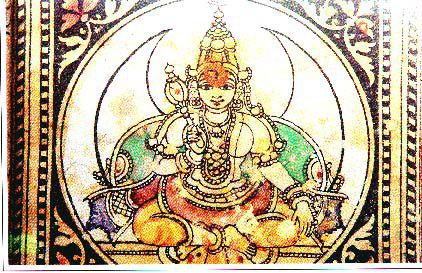
\includegraphics[width=0.5\textwidth]{pics/Moon_type.png}
 \end{figure}
 

Moon types are dominated by the water element and show the water element in its greatest flourishing. They have round faces and roundish well‑developed flesh or corpulent bodies. They have attractive faces, hair and features, particularly when young and can be quite beautiful, possessing a certain luminosity. With age they tend to become maternal types and put on weight and water. For women this often happens after the birth of the first child or after the age of thirty. They possess an abundance of vital fluids and have thick, shiny oily hair and skin. Their complexion is usually fair or whitish, and the whites of the eyes are pronounced. Lunar women usually have a good development of the breasts and thighs.

 

Moon types run cold and damp and can easily accumulate phlegm and mucus. They often develop water retention. They have strong lungs and good voices but often suffer from congestion. Usually they live long and are healthy, but may have some constant minor health problems. Often the kidneys are their weakest organ. They are prone to laziness or excessive sleep.

 

Psychologically speaking they are also maternal, loving, caring, nurturing and helpful to others. They are loyal and dependent and make good friends and marriage partners. They are good cooks and are domestically oriented. Their life is centered in home and family. Yet once they overcome their basic shyness and learn to relate on a public level they can succeed socially or politically and become good and sensitive leaders.

 

Moon types are highly emotional, romantic and sentimental and cry easily. Though they are easily hurt, they easily forgive and forget. Their emotional sensitivity is not always a real sensitivity to the emotions of others; sometimes they may be so caught in their own emotional responses that they cannot really see what others are feeling. Yet their emotional sensitivity may give them artistic talents, particularly for the performing arts.

 



\subsubsection{MARS TYPES}
 

 \begin{figure}[H]
 \centering
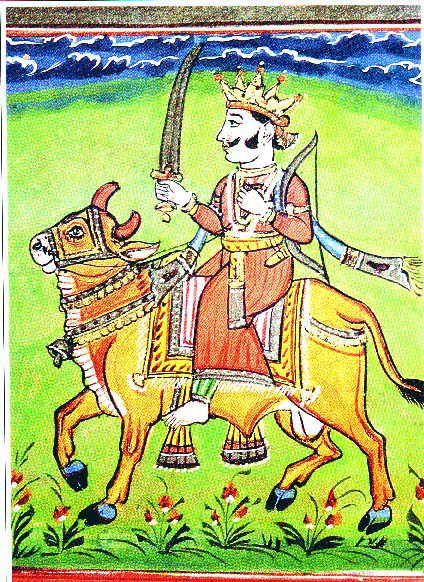
\includegraphics[width=0.5\textwidth]{pics/Mars_type.png}
 \end{figure}
 

Mars represents the negative side of the fire element and its excesses and diseases. While Sun types run hot and dry and maintain a good digestive power, Mars types run hot and wet. They get weakened digestion and easily come down with infectious diseases. They suffer from excess bile and acid. Their blood runs hot and they easily accumulate toxins. They tend towards disease, particularly of an inflammatory nature. They suffer from excess heat and dampness.

 

Generally, however, Mars types possess strong energy and have periods of very good health. But owing to bad living habits, they periodically suffer from acute diseases. They suffer from overuse of alcohol, cigarettes, meat, hot spices, oily and fried foods, overdrinking and overeating. Anger, jealousy and hatred damage their constitution. Usually the liver is their weakest organ and they tend hepatitis, cirrhosis and herpes.

 

Mars types are the most prone to injuries, accidents and traumatic diseases, generally from their own rashness or violent behavior. They often have surgeries or even organs removed. Disease comes to them from outside factors; their basic vitality is usually good. Their health problems are thus not so often necessary as due to their own excessive or blind actions.

 

Physically, Mars types possess moderate build with good muscles. Their complexion tends to be red, with oily skin and they bruise or bleed easily. Their eyes are often red and they tend towards eye diseases. They are sensitive to the sunlight and often wear glasses or sunglasses.

 

Psychologically, Mars types are perceptive, critical and argumentative. They are aggressive and persistent, bold, daring, rash and adventurous. They often get into arguments and conflicts. They make good debaters, speakers, and lawyers. Their sense of logic is strong but often follows their anger more than a real sense of justice. They love to win and hate to lose. Often they will do anything to win.

 

Mars types possess a good sense of mechanics and make good scientists, research workers and are good at working with tools and weapons. They need a practical outlet for their energy to prevent it from going to excess.

 

Mars types, however, are very loyal to their friends and like to form alliances, though usually as opposed to an external threat. They have strong passions and are very possessive. Their sexual energy is strong but not always refined. They tend to overindulge and burn themselves out.

 

A higher Mars type exists as well. This is the highly perceptive and self-disciplined yogi. They are ascetics who mortify their bodies and know how to control their minds. They possess a strong will towards transformation and are willing to pay the price for it.

 



\subsubsection{MERCURY TYPES}
 

 \begin{figure}[H]
 \centering
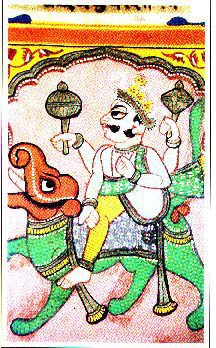
\includegraphics[width=0.5\textwidth]{pics/Mercury_type.png}
 \end{figure}
 

Mercury represents the positive side of the air element. Mercury types are very airy, intellectual and nervously sensitive. They are congenial, communicative and compassionate. They are very friendly but tend to be introverted from an excess of thinking. As Mercury is a mutable planet, they often take the physical appearance of the planet strongest to aspect Mercury.

 

Yet Mercury physical types do exist. They are a little tall or short, thin in build, and generally attractive. Their eyes are often greenish and their skin is a little moist, unlike other air types that tend to be dry. They run on the cool side and often have sensitive lungs. They are susceptible to allergies and hay fever as well as to bronchial disorders. Their digestion is often weak or variable. The heart is sensitive and they are prone to palpitations.

 

Mercury types possess good prana or life‑energy, live long, and have a certain glow. They are often athletic and make good runners or basketball players but their endurance is not always high. Often they are athletic when young but shift over to more intellectual pursuits after puberty.

 

Psychologically, Mercury types possess quick minds, a good sense of information and fluent powers of speech. They are good at languages and at statistics but may get their minds caught in trivia. They are witty and have a good sense of humor. They are helpful, service oriented and often take background or dependent roles. They are good at the mass media and make good moderators and interviewers. They may have powers of acting and are good at imitation.

 

Mercury types make good secretaries, teachers and writers. With their strong sense of consideration and their desire to create harmony in life, they also make good doctors and nurses. They love nature, particularly plants, and are good at gardening. They have a refined sense of taste usually free of sensuality. They can develop a deep spirituality once they learn to turn their minds inward.

 



\subsubsection{JUPITER TYPES}

 \begin{figure}[H]
 \centering
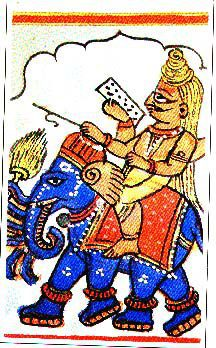
\includegraphics[width=0.5\textwidth]{pics/Jupiter_type.png}
 \end{figure}
 
 

Jupiter is the positive side of the water element. Jupiter types possess strong watery constitutions, with good muscles, flesh and fat. All their body tissues are well developed. They tend towards corpulence, mainly later in life, but are seldom much overweight. Their complexion is tinged yellow or golden. They often have great strength and love physical work, exercise and trips into the wilderness. Generally they are very healthy and long-lived. Their most weak organ is their spleen-pancreas. They suffer mainly from overeating sweet, rich and oily foods. Excessive sugar consumption can lead them to diabetes. 

 

Psychologically, Jupiter types are joyful, jovial and content. They tend to overindulgence or self‑complacency. They are friendly, generous and enjoy being with people. They have a strong sense of play and enjoyment, yet seldom become vulgar. They are kind and compassionate and always try to be just. Yet their sentiments and ideals may be too grandiose. They love music, enthusiasm and the display of energy. They are more active and athletic than the other watery types.

 

Generally, Jupiter types are highly moral and ethical people and are devoutly religious. However, they tend towards conventionality in their beliefs and do not like to offend anyone. They have a strong devotion, are the most calm of all types and can easily be at peace within themselves. They develop a contemplative or philosophical bent, as they love to find the larger forces at work in life and join the energy of expansion. Their spirit is positive, expansive and helpful. They seldom worry and tend towards over optimism. They have a natural interest in the spiritual life and in promoting higher causes.

 



\subsubsection{VENUS TYPES}


 \begin{figure}[H]
 \centering
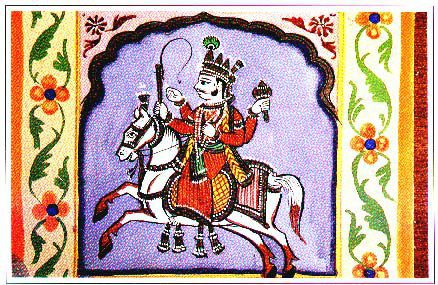
\includegraphics[width=0.5\textwidth]{pics/Venus_type.png}
 \end{figure}
 
 

Venus types are often beautiful, being the most attractive of all planetary types. They possess beauty of face, hair and eyes and a general sexual charm and artistic grace. Their tissues are roundish and well developed but they seldom become overweight. Their hands are well formed and delicate, without deep lines. Their sexual vitality is strong and they have somewhat feminine features, even in the men. Yet they have a certain strength and magnetism as well. Venus types are generally healthy, except when they over indulge themselves, in which case they suffer from weakness of the kidneys, reproductive organs, lungs and heart.

 

Psychologically, Venus types are romantically inclined, but not really sentimental. They feel the complementary nature of all forces in life. They have a strong sense of grace. They make good artists and possess a good sense of form and design. They possess good imaginations and have vivid dreams. Their disposition is generally ethical and they possess love and devotion. They are strongly socially minded.

 

Venus types love beauty, comfort and elegance and like to adorn things, including, first of all, their own bodies. They enjoy jewelry and like beautiful homes. They love to display the beauty they possess and to charm others. As such, they can become addicted to luxury but are seldom really greedy. They have a good spiritual potential once they learn the meaning of Divine love. They have good occult or astrological insight through appreciating the beauty of natural law.

 



\subsubsection{SATURN TYPES }


 \begin{figure}[H]
 \centering
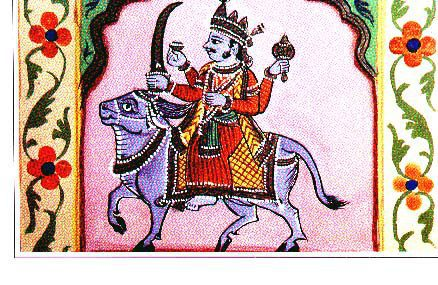
\includegraphics[width=0.5\textwidth]{pics/Saturn_type.png}
 \end{figure}
 
 

Saturn types are usually the least attractive of planetary types. They are unusually tall or short, thin and bony. They may have large noses or large teeth, with unrefined countenances. Their hands and feet tend to be large. Their skin is dry, rough or cracked and tinged brown or black. Their hair is brittle; their nails may be cracked. A more attractive Saturn type does exist, usually as an artist with some Venus influence. The person is dark, elusive, gaunt and striking in appearance.

 

Saturn types are the most disease-prone of all planetary types. They have usually low vitality, poor endurance, and cannot handle much stress. They run cold and have poor digestion and poor circulation. They tend towards constipation and to accumulate waste materials in the body. They are often chronically ill and may pass away prematurely.

 

Psychologically, Saturn types are saturnine. They are overly serious, even morbid. They are usually pessimistic and may suffer from depression. They are generally introverted, solitary and often selfish. The many difficulties that they face in life make them insensitive to the needs of others. They may be miserly and overly calculating. As what they gain only comes through much effort, they are unwilling to share it. They tend toward worry, fear or anxiety, seldom smile and are rarely really happy. They are practically-minded and seldom good dreamers or inventors.

 

Higher Saturn types are yogis, ascetics or monks who renounce the world. They possess detachment and are free of emotional fluctuations. They are beyond the cares of the world. Other Saturn types may be rebels or artists who stand outside of society. Saturn tends to make us unorthodox or non-conformist. Lower types, on the other hand, may be criminals, underworld figures or tyrants (particularly when the influence of Saturn combines with that of Mars). They are suspicious and paranoid, greedy and selfish.

 



\subsubsection{RAHU TYPES}


 \begin{figure}[H]
 \centering
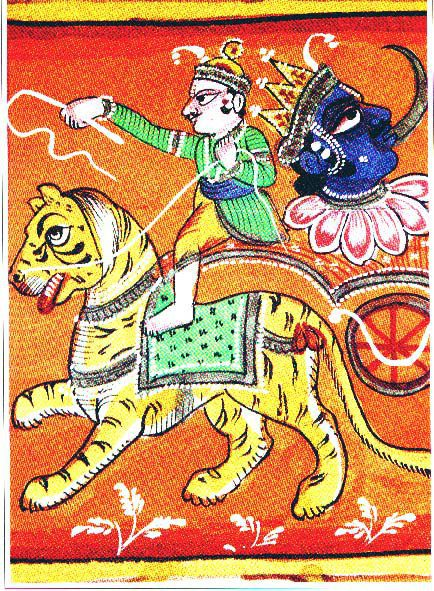
\includegraphics[width=0.5\textwidth]{pics/Rahu_type.png}
 \end{figure}
 
 

As Rahu and Ketu are not really planets, one may think that planetary types for them do not exist. Yet they can be delineated at least as secondary types. They do have powerful influences on our mind and character, which affects the physical body as well.

 

Rahu types are often born near an eclipse of the Sun or Moon or at the time of the new Moon. They are dark in features and mobile, moody and changeable in temperament. There is a kind of cloud around them, a dark shadow and they have deep-seated psychological problems from the past haunting them. They are a little ghostly in their manners and appearance.

 

Rahu types possess very sensitive nervous systems and often suffer from insomnia or nightmares. On a psychic level, they are partly possessed by something, another entity, curses or unfulfilled longings from past lives. While they easily gain psychic, occult and astral sensitivities, it can be dangerous for them. They may become mediums or do channeling but are easily caught by illusion. Their mental control is tenuous at best.

 

Rahu type women are very clinging but at the same time very willful and like to control their men through crying, hysteria or even threats of suicide. They exert a strange fascination over men that proves destructive. They are tempting, strangely fascinating and alluring.

 

Rahu individuals possess grandiose desires or insatiable cravings, but are incapable of accomplishing ordinary things. When they have success in the world, it is unfulfilling and may cause mental breakdowns or other psychological problems. Their egos are inflated but weak. They are either dominating or dominated. They suffer from a certain vanity and have unrealistic fantasies. Spirituality comes to them only after a great deal of self-examination and learning of self-control.

 



\subsubsection{KETU TYPES}
 

Ketu types are introverted and individualistic to the point of eccentricity. They go their own way and rebel against the social order. Often they debase themselves by following lower social influences. They possess self‑doubt and even while they go their own way, they are confused about what it really is. They are very sensitive to criticism and react in a strongly defensive manner. They often suffer from neuromuscular disorders and have a lack of coordination. They are prone to accidents, surgery, or violence and suffer in wars and other mass catastrophes.

 

Ketu types are perceptive but their focus is narrow. Their minds are critical, negative and highly discriminating. They tend to be overly serious and are seldom really happy. They are often fixated on the past and may make good historians or archaeologists. They are probing, searching and examining. Once a problem enters their minds they will go over it endlessly until they find an answer. Often they are so doubting that they never arrive at an answer or if one comes, they do not trust it. They are best at obscure research and are able to find the light in darkness, though they may miss the light of day.

 

Higher Ketu‑types are yogis (Jnanis) and possess much spiritual knowledge and insight. They see the illusory and transient nature of the world and go their own way regardless of circumstances. They are free of karma and desire. They are able to see through and go beyond the ego. They are a law unto themselves. They may not be recognized or appreciated but they are beyond the praise or blame of the world.

 

 

\subsection{SUMMARY OF PLANETARY TYPES}
 

We can ascertain all the variations in human types in planetary terms. We can understand all human problems according to the energetics of the planets. We can determine all psychological problems according to the functioning of the planets on a lower level, and spiritual growth as their function on a higher level. Yet for this we have to look deeply at the planets and not just according to stereotypes.

 

The key to inner growth is to move from the lower to the higher functioning of our planets. This is to become conscious of their workings and their potentials on both inner and outer levels. It also requires an integration of the planetary influences within us.

 

\subsubsection{DUAL PLANETARY TYPES}

 

For people who have two planets of equal strength, a mixed type will emerge. For example, a Sun-Moon type will have a strong personality, both in its active and receptive, solar and lunar sides. A Mars-Jupiter type will give a Jupiterian expansiveness to the Mars work and action principles. A Mercury-Jupiter type will have an expansive but detailed and strong intelligence. A Mars-Venus type will have a strong sexuality, passion and vital will.

 

Sometimes higher and lower planetary influences combine as well. For example, a person may have a higher Jupiter influence with a lower Mars energy. They may have much expansiveness, faith and a philosophical disposition but allied with a lower Martial will to impose it upon others.

 

\subsubsection{SECONDARY TYPES}

 

Secondary planetary types also exist. A person may be primarily Moon but Venus secondarily, for example. They will have a strong lunar, maternal or receptive feeling nature, yet with a significant need for affection and beauty, Venus traits. Another person may be primarily Moon but secondarily Mercury. They will be intellectual, poetic and socially minded.

 

Thus, we can understand the differences between people of the same planetary type by what planet is second in their nature. This affords us much more specificity in our interpretations.

 

\subsubsection{WEAK PLANETARY TYPES}

 

Sometimes a weak planet characterizes a person – they can be seen by the planetary strengths lacking in their nature. For example, if the Moon is weak in a chart, fear, moodiness and an inability to relate to people will characterize the person. Such an influence may be so strong that it is best to aim at correcting this weak planet rather than dealing with the planetary type.

 

Most often, however, weakness of a planet is caused by another planet being too strong or pronounced. For example, a strong or prominent Saturn and Rahu and their malefic influence are usually behind a weak Moon. Hence, Saturn or Rahu types usually have weak Moons.

 

\subsubsection{INDEX OF PLANETARY INFLUENCES }

 

While the basic planetary type is crucial, we must remember that each of us contains the influences of all the planets. Through Vedic Astrology, we can examine the relative strength and weakness of all the planets. This includes two main factors:

 

The first and most significant factor is the general strength of the planet by house, sign and aspect.
The second is the friendship and enmity between planets, particularly that between the planet and the ruler of the sign in which it is located (its dispositor).
 

Whenever we examine a chart for a person we should help them understand not only their planetary type but the general meaning of all the planets and their relative strength or weakness of their chart overall. In the end, each chart, like a painting, will have its own design and special way to understand it. Houses, signs and planetary periods also strongly color our lives. Yet one planet will usually stand out, either as the planetary type or the dominant planetary influence for a giving time or given concern.